\documentclass[10pt,a4paper]{report}
\usepackage[latin1]{inputenc}
\usepackage{amsmath}
\usepackage{amsfonts}
\usepackage{amssymb}
\usepackage{graphicx}
\usepackage{url}
\newcommand{\black}{\texttt{Black}}
\newcommand{\white}{\texttt{White}}
\newcommand{\loc}[1]{\texttt{#1}}
\author{James Pettit}
\title{Simulation Learning in Computer Hex}
\begin{document}
\maketitle
\tableofcontents

\chapter{Introduction}
Abstract strategy games provide an easy testbed for artificial intelligence and machine learning applications. The game framework provides immediate feedback on algorithm performance. The choice of game and rules can also be experimentally chosen for a variety of difficulty and computational complexity levels. Starting with mathematical game theory research, the most common technique for game AI has been brute force search of the tree of legal moves. This technique, highly tuned and optimized, is what led to Chinook's ascendance to World Champion in 1994 and Deep Blue's eventual victory in 1997 over then World-Champion Gary Kasparov. These victories cemented brute force tree search as standard techniques in abstract strategy games, to the point where computers constructing endgame tables have been strong enough to find sequences lasting for hundereds of moves. Kasparov himself suggested a version of Chess that allowed the player to consult a computer for move advice. Chinook went so far as to solve checkers, proving that perfect play will end in a draw. For at least Checkers, Chess, and similar games (Othello, Connect Four), brute force tree search has provided a silver bullet.

\section{Background: The Game of Hex}
Hex is a two player, full-information, abstract strategy game played on an $N$x$N$ grid of hexagons. The players are denoted by colors here \black{} and \white. The object of the game is to form an unbroken chain from one side of the board to the other. \black{} attempts to connect top to bottom, \white{} left to right. Figure \ref{fig:13x13inprogress} shows an example game in progress on a 9x9 board. Figure \ref{fig:13x13finished} shows a different game, where \black{} has just played the winning move, with an unbroken chain connecting top to bottom. Hex has properties that make it attractive for AI research. Once placed, a piece never leaves the board. The only criterion for a legal move is that the point be unoccupied (empty). Gale '79 proved the game cannot end in a draw, simplifying minimax methods. Nash, one of the inventors of the game, used a strategy stealing argument to prove the existence of a winning strategy for the first player, but the proof is by reduction and offers no insight into the strategy itself. Solutions for all opening positions for 7x7 and 8x8 boards have been found\cite{henderson2009solving}. A good portion, but not all, 9x9 openings have also been solved. Nash proposed 11x11 as the ideal board size, but 13x13 has been more common in competitions, especially as the ability of computer players improves.

Three Hex programs are currently in the running as viable world champions. Gabor Melis' \emph{Six} is the previous world champion (up to 2007). Six uses traditional alpha-beta search with and evaluation function based on an electical circuit model (proposed by Anshelevich 2002)\cite{anshelevich2002hierarchical}. \emph{Wolve}, from the University Alberta, also uses the Anshelevich algorithm, but more aggressively prunes provably inferior moves. \emph{MoHex}, also from Alberta, is based on the newer Monte-Carlo Tree Search technique, leveraging the open source \emph{Fuego} library. MoHex is the current world-champion, having finished ahead of Wolve in 2009 and 2010.

\begin{figure}
	\begin{center}
	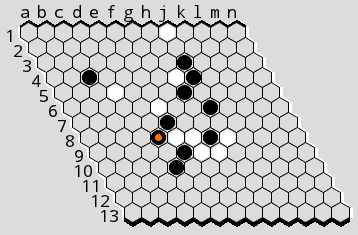
\includegraphics[width=200px]{graphics/13x13-in-progress.png}
	\caption{13x13 Hex Game, \white{} to play.}
	\end{center}
	\label{fig:13x13inprogress}
\end{figure}
\begin{figure}
	\begin{center}
	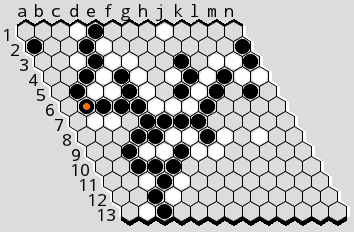
\includegraphics[width=200px]{graphics/13x13-finished.png}
	\caption{Finished 13x13 Hex Game, \black{}'s play at \loc{b6} gives him an unbroken path from top to bottom.}
	\end{center}
	\label{fig:13x13finished}
\end{figure}

\section{Overview of the Thesis}\label{overview}
In Chapter \ref{mcts} we will start with the current state of the art in Monte Carlo Tree Search (MCTS). MCTS is a technique to stochastically sample paths through a game-tree. It has been found to work well in games where: the tree is too large to consider brute-force search, no good solution exists to prune ``bad'' nodes, and no good evaluation function exists. Section \ref{bias} covers the current methods of biasing the tree search, including some methods similar to the technique presented in this paper. Chapter \ref{problem} covers why finding a generic way to bias the tree search would be a step forward in MCTS, with a formal definition of biasing the search, allowing a comparison of different but similar techniques. Chapter \ref{solution} presents a way of biasing the tree that can be automatically evolved through self-play, and does not require outside ``expert'' knowledge. Finally Chapter \ref{results} summarizes the technique and its usefulness, and discusses what can be done in the future to improve and extend it.

\chapter{State of the Art in Monte Carlo Tree Search}\label{mcts}
As stated, the current top computer Hex player, MoHex, uses the open-source Fuego implementation of Monte-Carlo Tree Search (MCTS). The basic Monte-Carlo technique for Computer Go was proposed by Bru\"{u}gmann\cite{brugmann1993monte}. His program \emph{Mango} effectively used a ``flat'' search tree (1-ply) and simply ran simulations from each candidate move to estimate its value. To contrast, MCTS uses Monte-Carlo simulations to grow a minimax search tree. The UCT algorithm was developed alongside MCTS to direct the growth of the search tree\cite{gelly2006exploration}. At any point, the search can be stopped and the current state of the tree used to select a move to play. Performance of the search is primarily based on three factors: the \emph{selection policy}, the \emph{simulation policy}, and the \emph{update policy}.

All nodes in the tree corrospond to a fixed position, i.e. the occupancy state of the board and which player is next to move. Nodes also have statistics associated with each position - the number of winning simulations performed that used the node, and the total number of simulations that included the node. In general, at each iteration the algorithm will, starting at the root node, recursively traverse the tree until it reaches a leaf node whose estimated value is unknown. A simulation is run from the position of this leaf node and the result used to update all nodes along the path. The algorithm continues for some set number of iterations, each iteration corrosponding to one simulation.

\begin{verbatim}
function search(root):
  for i in range(simulations):
    step(root)
		
function step(node) returns outcome:
  if node.visits < threshold:
    outcome = simulate(node)
  else:
    next = select(node)
    outcome = step(next)
  if outcome is win for node's player:
    node.wins++
  node.visits++
  return outcome
\end{verbatim}

\subsection{Selection Policy}
The \texttt{select} function defines the selection policy. It must return the child of the given node the step into next. In general, selection must trade off between \emph{exploitation} and \emph{exploration}. It is advantageous to exploit child nodes with high win-rates, to discover possible weaknesses that would result in the opponent winning. Simultaneously, a node with a low win-rate might only have had a few unlucky simulations run through it, resulting in an incorrect value estimate. Nodes with a low number of visits must be explored to see if they result in a high-value position.

One function that balances this trade-off is Upper-Confidence for Trees (UCT). UCT incorporates the win-rate of a child with a term that increases in value as the ratio of the child's visits to its parents decreases. Eventually, no matter how bad the estimated value of a position is, it will be re-visited and the estimate updated. UCT has several variations, but the ``pure'' version has been proven to eventually yield the correct minimax value of a position, given an infinite number of simulations\cite{gelly2006exploration}.

\[
	\texttt{winrate} + C*\sqrt{\frac{\log{(\texttt{parent.visits})}}{\texttt{child.visits}}}
\]

$C$, the \emph{exploration coefficient}, can be varied to increase or decrease the level of exploration versus exploitation. Note that a very low value will yield a function that relies almost exclusively on the estimated win-rate of a position, while a high value will visit nodes more equally, placing less emphasis on the estimated value.

\subsection{Simulation Policy}
The \texttt{simulate} function plays out the rest of the game from the current position. The simplest policy plays a legal uniform random move until the game ends (in Hex, when one player has a winning path). The simulation policy has the largest effect on the strength of the entire search. Initial research in Computer Go focused on using a strong simulation policy, using expert-derived heuristics to select the next move. The top Computer Go programs all have complex hand-crafted policies with rules to examine the current position and select a ``good'' move to play, possibly with a stocastic choice between several candidates. Only when none of the rules match do they fall back to a uniform random move. It was quickly found that building a stronger simulation policy does not guarantee better performance when used in the full tree search. A test and check methodology is required, with changes to the simulation policy having unpredictable effects on overall performance.

Recent research has focused on learning a simulation policy...

\subsection{Update Policy}
AMAF/RAVE

\section{Biasing the Tree}\label{bias}
In general, there are three ways to bias the tree search. First, upon expansion of a node, an initial estimate of the node's value is used. Over time, the initial estimate is gradually replaced RAVE and progressive bias are examples 

Mogo and others showed that using heuristics in both the expansion and playout policy can prove extremely beneficial. However, this requires expert knowledge (heuristics) that can be hard to obtain or not available for some games (particularly new games). It was also found that just improving the playout policy to play better was not enough. The playout policy can implicitly prune good moves, never allowing them to be played. If there is some small probability of playing a purely random move, the convergence properties of the MCT search will still hold, but can require a prohibitive amount of playouts to ``find'' the move sequence. Biasing tree expansion has similar problems. If the initial value estimate is incorrect, the selection policy will eventually expand the node enough times to find a winning sequence, but in practice the heuristics can hurt performance.

\chapter{Problem Statement}\label{problem}
Want to find a way to learn how to bias the search. Hand-crafted heuristics are tedious and don't extend to new games. Learning heuristics from expert games can be automatic, but requires a corpus, again, can't be used on new games.

\chapter{Solution}\label{solution}

\section{Evolution Strategies}
Evolution strategies (ES) is a collection of algorithms that operate on real-valued vectors. A general form of ES is given here, with some small modifications required for it to represent a biased simulation policy discussed in Section \ref{esmods}. More information on evolution strategies and evolutionary learning in general can be found in Eberhard and Shi's excellent textbook \emph{Computational Intelligence: Concepts to Implementations}\cite{eberhart2007computational}. The Evolution Strategies article on Scholarpedia.org also provides a good introduction to the topic\cite{Beyer:2007}.

\begin{enumerate}
\item A population (usually 20-200 individuals) is generated. In ES, each individual is represented by its vector, often called its ``position'' ($\bf{p}$), a single real-valued ``strategy'' ($\sigma$), and, once evaluation is complete, a single real-valued ``fitness'' attribute ($f$).
\item The algorithm loops, each loop forming one ``generation'':
	\begin{enumerate}
	\item From the $\mu$ parents, generate $\lambda$ children.
		\begin{enumerate}
		\item Each child is created by selecting $P$ parents.
		\item These parents (usually 2 or 3) are \emph{recombined} by averaging their positions component-wise to form the new child position. Similarly, the child's strategy is the average of its $P$ parents.
		\item	The child's strategy ($\sigma$) is \emph{mutated} by a Gaussian distributed random variable.
		\item The child's position is mutated component-wise by a vector of iid Gaussians, one per component of the dimension. These Gaussians are scaled by the strategy. Thus, one individual may mutate more (faster) than another, by using a larger strategy. These strategies mutate along with the positions, allowing the system to evolve the correct mutation weight along with the position.
		\end{enumerate}
	\item The best $b$ performing parents are propagated through without mutation, replacing $b$ children. This is done to preserve well-performing solutions.
	\item Evaluate the fitness of the $\lambda$ children (see \ref{fitness}).
	\item Sort the children by fitness.
	\item Cull the children by selecting only the top $\mu$. These now form the next generation of parents.
	\end{enumerate}
\end{enumerate}

Figure \ref{mutate} shows the differential equations for this evolutionary update. Note that $\sigma$ is multiplied at each time step, and can never reach zero. $\tau$, often called the ``learning rate'', can be scaled up or down to increase or decrease the variance of $\sigma$, a high values will give more mutation, low values less. The initial value of $\tau$ is $\frac{1}{\sqrt{2D}}$, $D$ the dimensionality of the search space. The rate decreases over time, as the number of generations approaches a set maximum, this forces the algorithm to converge, though not necessarily on a suitable solution. This choice of $\tau$ is driven by experimental literature suggesting it works in many cases\cite{Beyer:2007}.

\begin{figure}
\begin{flalign*}
	\tau_{t} = & \frac{1}{\sqrt{2D}} \left(1 - \frac{\textrm{generation}}{\textrm{max generations}}\right) \\
	\sigma_{t} = & \sigma_{t-1} e^{N(0, \tau^2)} \\
	p_{i_{t}} = & p_{i_{t-1}} N(0, \sigma^2)
\end{flalign*}
\caption{Differential equations for $\tau$, $\sigma$, and $\bf{p}$, indexed by time $t$. $D$ is the number of dimensions, i.e. $|\bf{p}|$}
\end{figure}\label{mutate}

\section{Using ES to Bias a Simulation}\label{esmods}

\section{Fitness Evaluation}\label{fitness}

\chapter{Results and Conclusions}\label{results}
\begin{itemize}
\item uniform local vs. control: 69.33\%
\item uniform local with tenuki vs. control: 61.33\%
\item learned local vs. control: 77.63\%
\item uniform local with tenuki vs. uniform local: 45.33\%
\item learned local vs. uniform local: 73.68\%
\item learned local vs. uniform local with tenuki: 75.00\%
\end{itemize}

Learned local play is the clear winner. Interestingly, the addition of a tenuki probability lowers performance in all cases. As expected, uniform local play significantly improves upon pure random playouts. The fact that evolutionary learning can find weights that boost performance versus uniform local in the same manner that uniform local improves upon pure random shows how much further there is to go, and shows the weaknesses of purely random simulations.

\bibliography{thesis}
\bibliographystyle{plain}
\end{document}
